\documentclass[crop,border=2pt]{standalone}

\usepackage{mathtools}
\usepackage{tikz}
\usetikzlibrary{positioning,scopes,arrows,shapes,decorations.pathreplacing}

\begin{document}
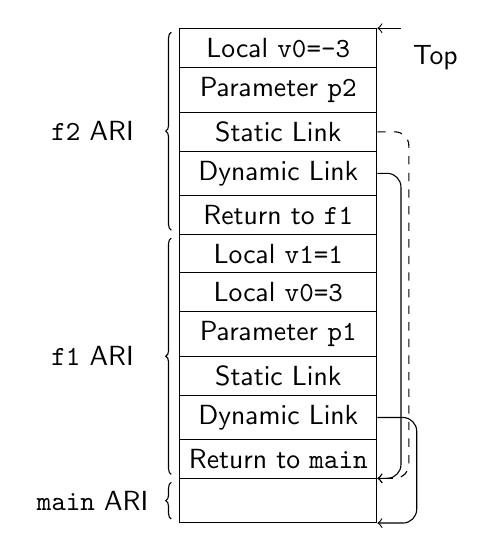
\begin{tikzpicture}[font=\sffamily,
  mystack/.style={rectangle split,rectangle split parts=#1,draw,anchor=center},
  myline/.style={->, rounded corners=5pt},
  dynamiclink/.style={myline},
  staticlink/.style={dynamiclink, dashed},
  mydec/.style={decorate,decoration={brace,amplitude=2pt}}]

  \node[mystack=12] (stk) {
    Local \texttt{v0=-3}
    \nodepart{two}Parameter \texttt{p2}
    \nodepart{three}Static Link
    \nodepart{four}Dynamic Link
    \nodepart{five}Return to \texttt{f1}
    \nodepart{six}Local \texttt{v1=1}
    \nodepart{seven}Local \texttt{v0=3}
    \nodepart{eight}Parameter \texttt{p1}
    \nodepart{nine}Static Link
    \nodepart{ten}Dynamic Link
    \nodepart{eleven}Return to \texttt{main}
    \nodepart{twelve}\phantom{Dummy}
  };

  \draw[dynamiclink] (stk.four east) -- ([xshift=.3cm]stk.four east) -- ([xshift=.3cm]stk.eleven split east) -- (stk.eleven split east);
  \draw[dynamiclink] (stk.ten east) -- ([xshift=.5cm]stk.ten east) -- ([xshift=.5cm]stk.south east) -- (stk.south  east);

  \draw[staticlink] (stk.three east) -- ([xshift=.4cm]stk.three east) -- ([xshift=.4cm]stk.eleven split east) -- (stk.eleven split east);

  \node [right=2.5cm of stk.text] (top) {Top};
  \draw[myline] ([xshift=.3cm]stk.north east) -- (stk.north east);

  \draw[mydec] ([xshift=-.1cm,yshift=.5mm]stk.five split west) --
               ([xshift=-.1cm,yshift=-.5mm]stk.north west) node [black,midway,xshift=-1cm] {\texttt{f2} ARI};
  \draw[mydec] ([xshift=-.1cm,yshift=.5mm]stk.eleven split west) --
               ([xshift=-.1cm,yshift=-.5mm]stk.five split west) node [black,midway,xshift=-1cm] {\texttt{f1} ARI};
  \draw[mydec] ([xshift=-.1cm,yshift=.5mm]stk.south west) --
               ([xshift=-.1cm,yshift=-.5mm]stk.eleven split west) node [black,midway,xshift=-1cm] {\texttt{main} ARI};

\end{tikzpicture}
\end{document}
